\chapter*{Fairness in income distribution}
\stepcounter{chapter}


\section{Overall Distribution of Income:}
\begin{figure}[H]
    \centering
    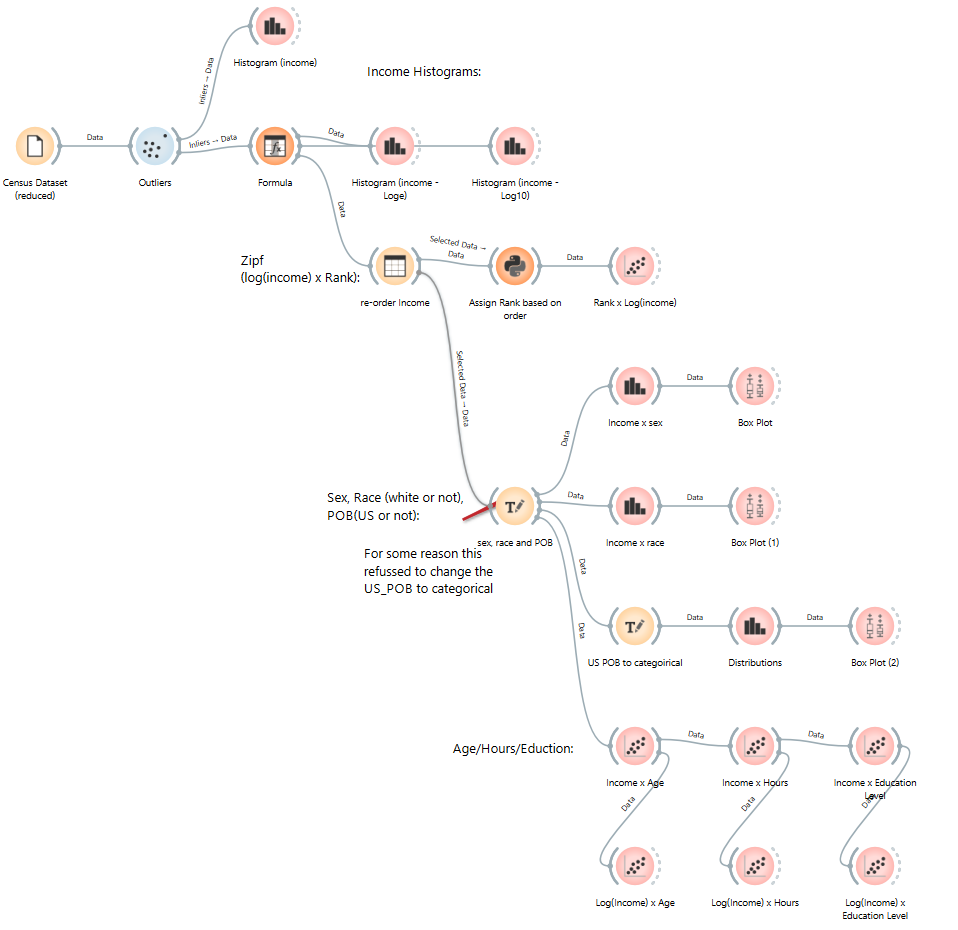
\includegraphics[width=0.7\textwidth]{chapters/part 2 - images/nodes.png}
    \caption{How the data was extracted.}
\end{figure}

\begin{figure}[H]
     \centering
     \begin{subfigure}[b]{0.45\textwidth}
         \centering
         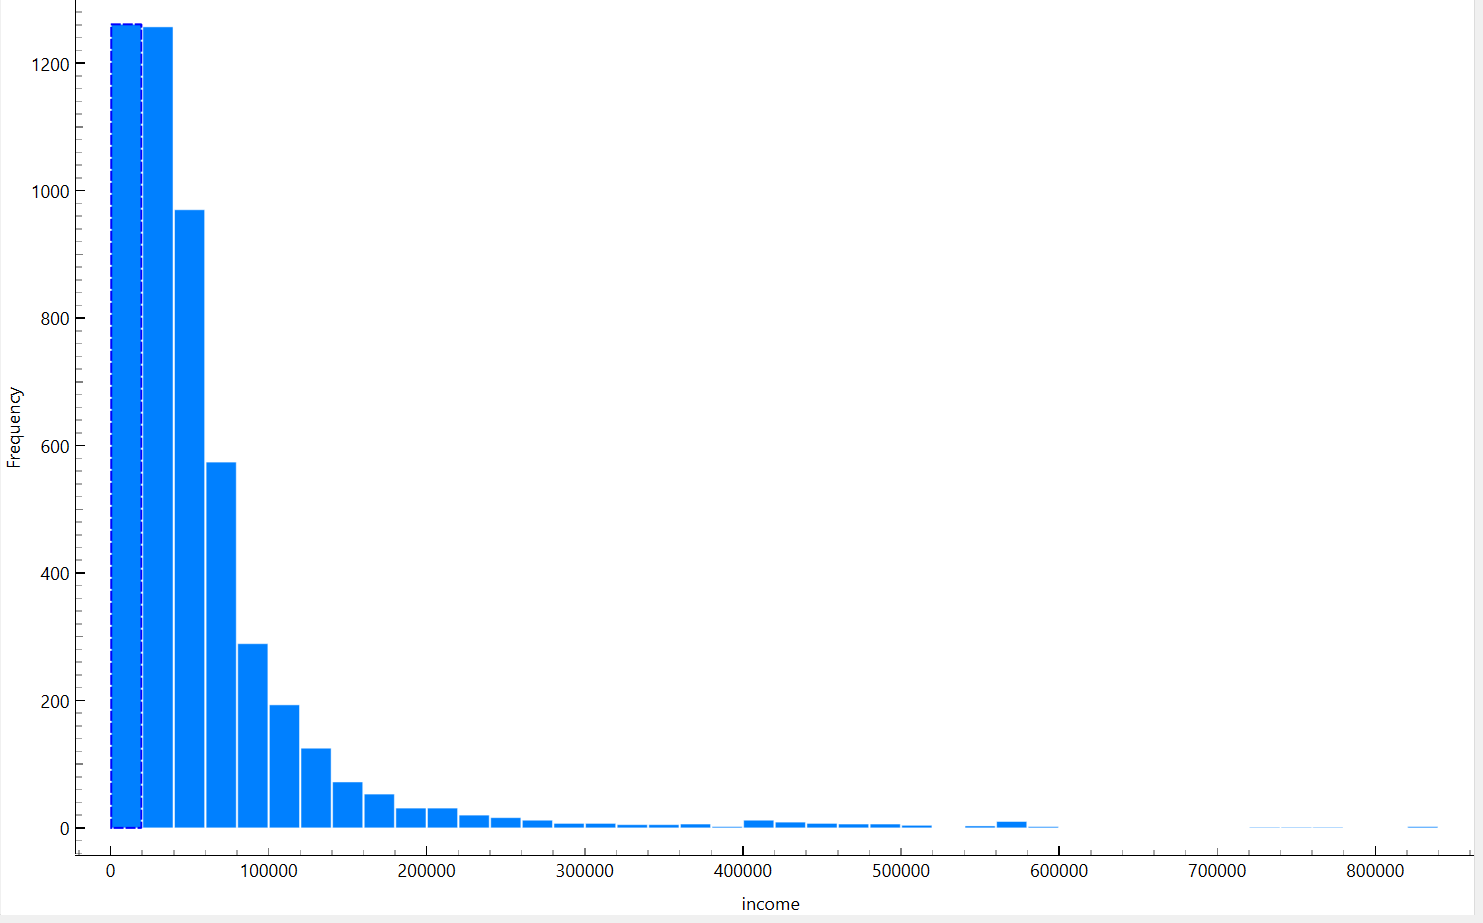
\includegraphics[width=\textwidth]{chapters/part 2 - images/raw_income.png}
         \caption{Raw Income Distribution.}
         \label{fig:raw_income}
     \end{subfigure}
     \hfill
     \begin{subfigure}[b]{0.45\textwidth}
         \centering
         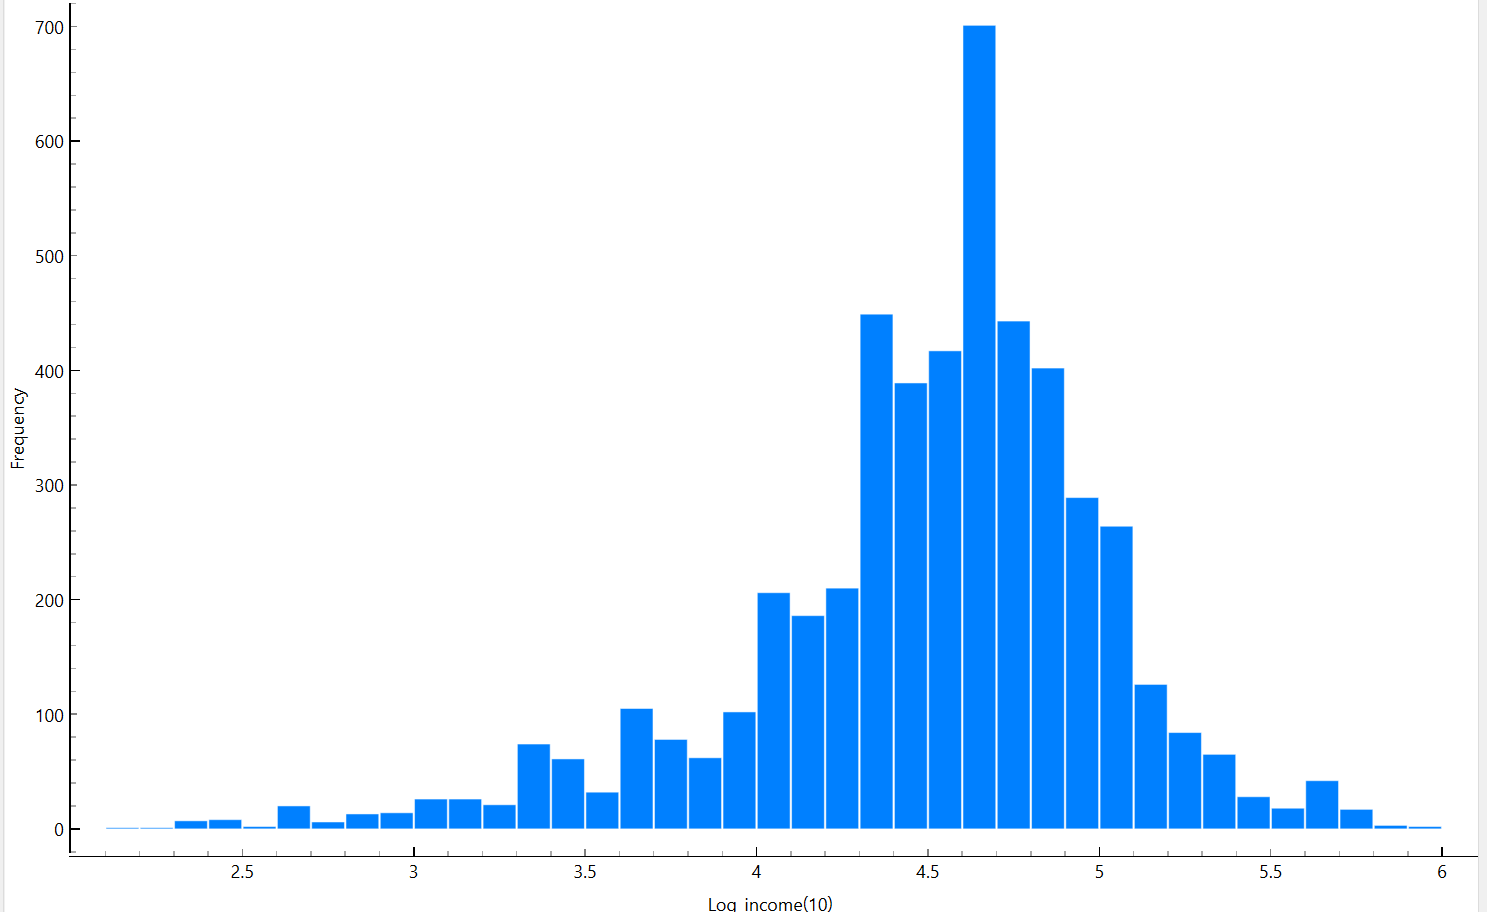
\includegraphics[width=\textwidth]{chapters/part 2 - images/log(income)-10.png}
         \caption{Income distribution using $\log_{10}$ scale.}
         \label{fig:log_income}
     \end{subfigure}
     \caption{Comparing income distribution metrics.}
     \label{fig:income_overview}
\end{figure}
As seen in Figure \ref{fig:raw_income}, the income distribution is more \textbf{reciprocal} in nature
as shown by its positive skewness. This is a result of most individuals earning in the lower brackets, with higher
paying jobs being distributed more sparsely.
To linearise this distribution and break down the $1/x$ relationship, a $\log_{10}$ transformation is used. This
base was chosen over the natural logarithm ($\ln$) because it provides a more intuitive scale for financial data.

\subsection{Additional notice:}
\begin{figure}[H]
    \centering
    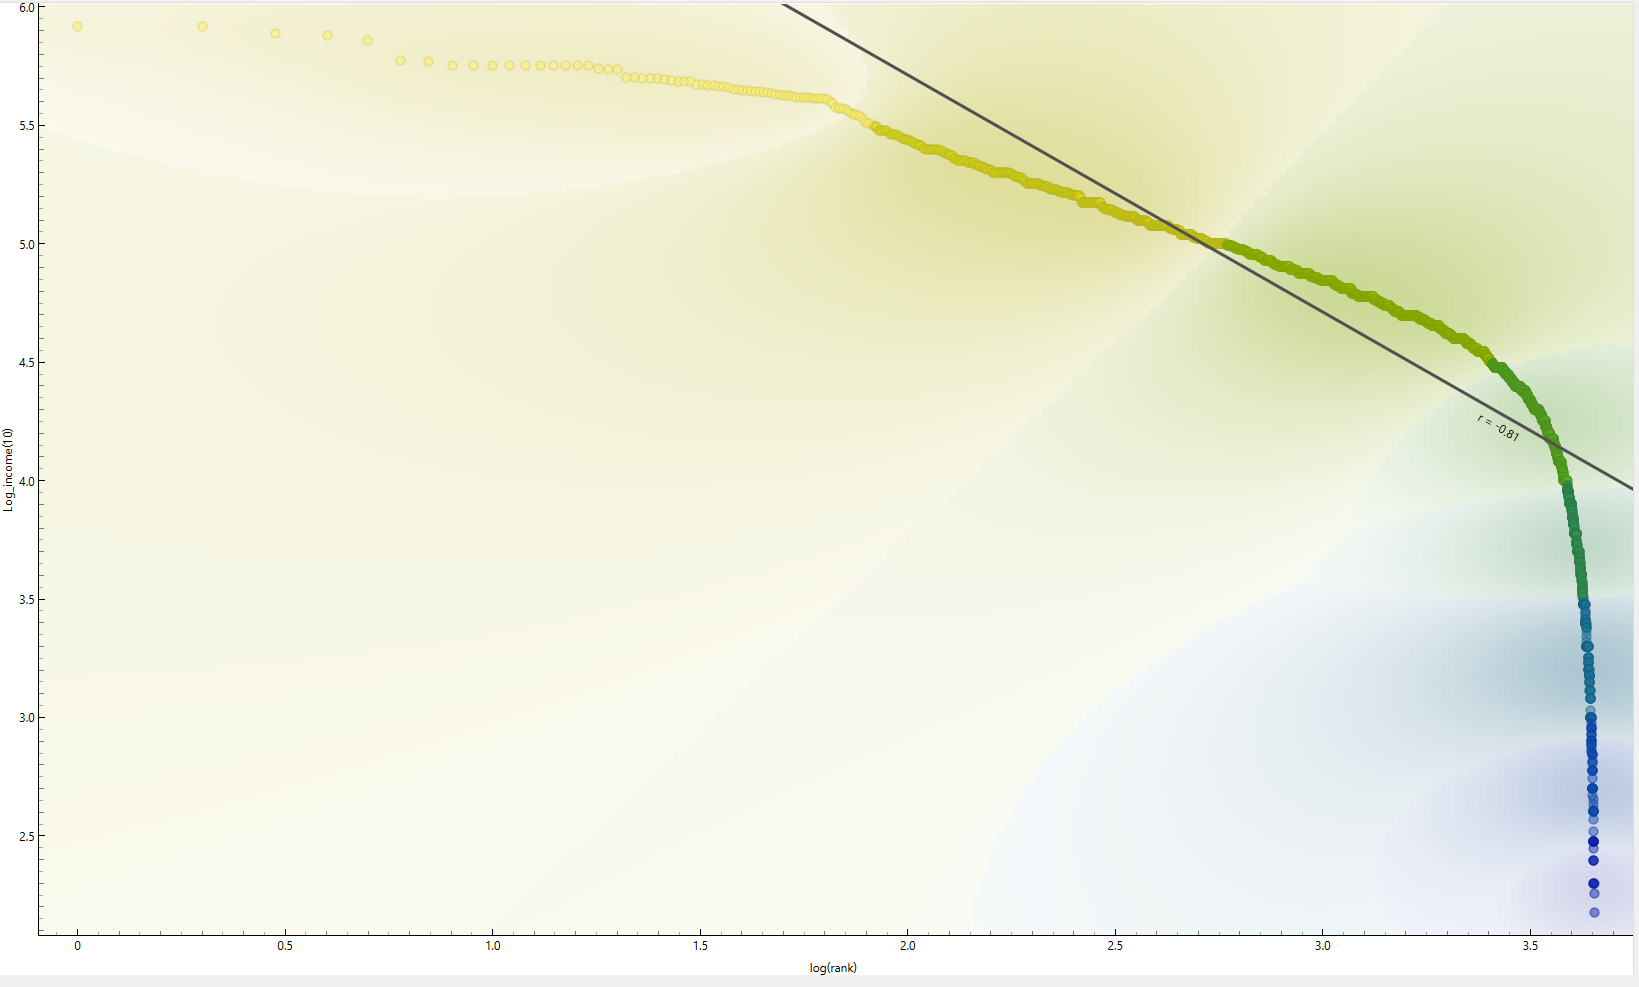
\includegraphics[width=0.7\textwidth]{chapters/part 2 - images/log(rank)_log(income).png}
    \caption{Log(income) vs log(income ranks)}
    \label{fig:wealth_dis}
\end{figure}
Another way to see how wealth is distributed is shown through a Zipf Plot (Figure \ref{fig:wealth_dis}). The
negative slope suggests that income drops off rapidly as rank increases, demonstrating a high concentration
of wealth among top-tier individuals. The plateau at the lowest ranks (top-left) represents the highest earners,
while the sharp descent toward the higher ranks illustrates how income diminishes for the majority of the
population. The $r = -0.81$ correlation confirms a strong inverse relationship between rank and income,
with the log-log representation confirming that the data follows a Pareto distribution (based on the idea that
a small proportion of instances hold a lot of the value within the data - few people earn a lot of money).

\section{Effect of \textbf{Sex} on Income distribution:}
\begin{figure}[H]
     \centering
     \begin{subfigure}[b]{0.45\textwidth}
         \centering
         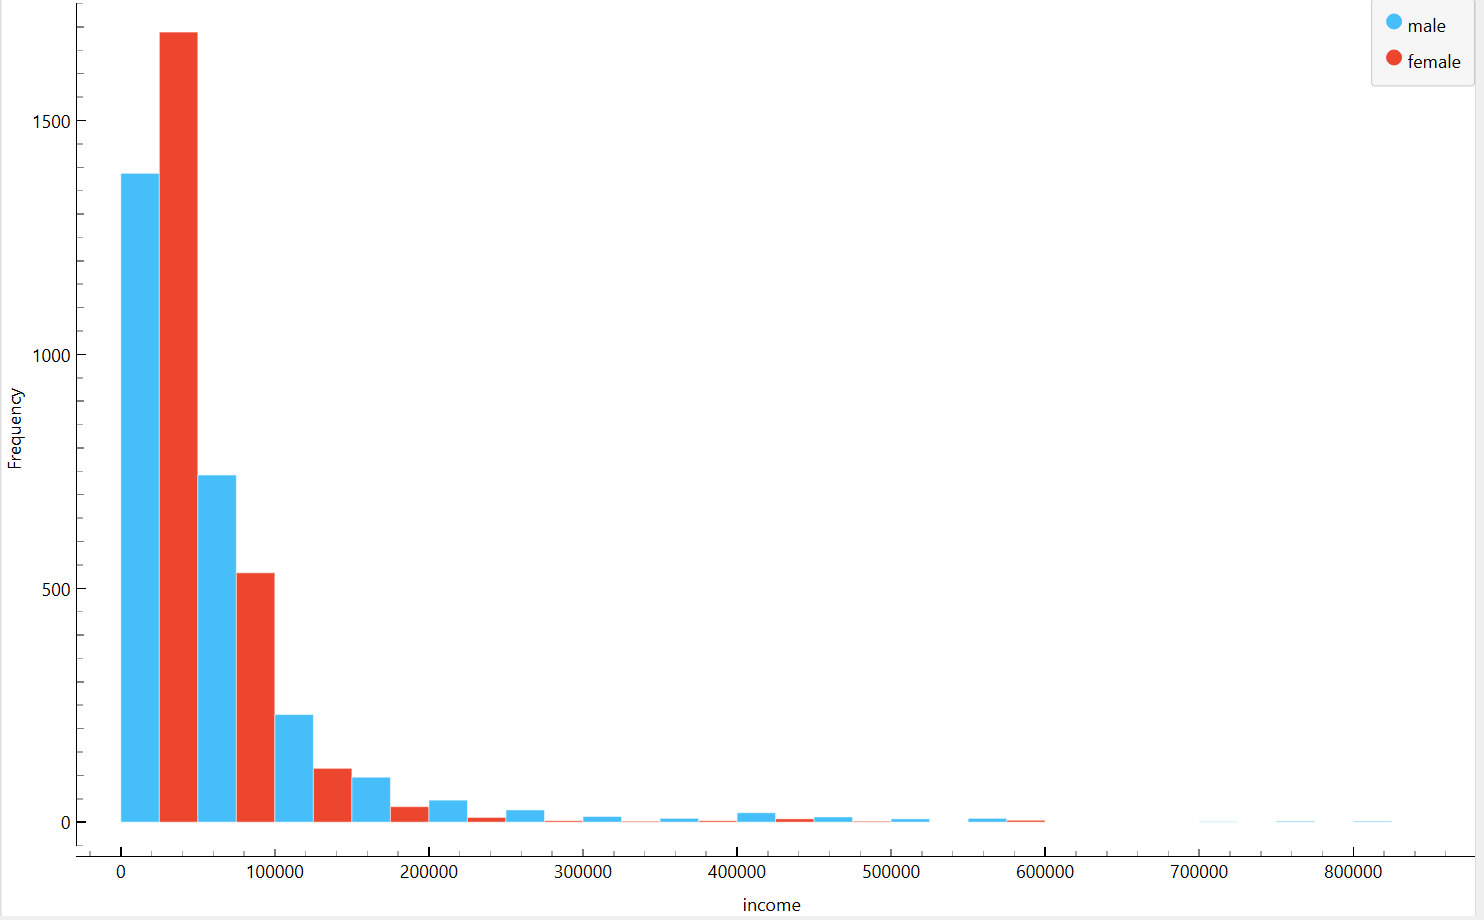
\includegraphics[width=\textwidth]{chapters/part 2 - images/income_sex_distribution.png}
         \caption{Distribution of Sex with Income.}
         \label{fig:income_sex_dis}
     \end{subfigure}
     \hfill
     \begin{subfigure}[b]{0.45\textwidth}
         \centering
         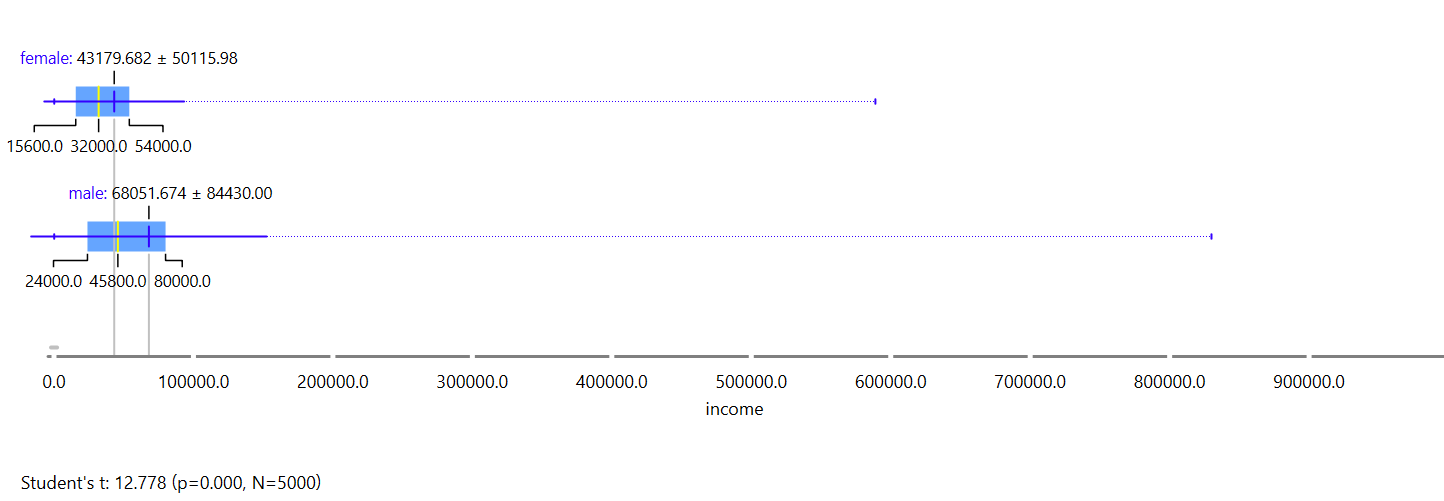
\includegraphics[width=\textwidth]{chapters/part 2 - images/income_sex_box.png}
         \caption{How does gender affect the distribution of income.}
         \label{fig:income_sex_box}
     \end{subfigure}
     \caption{Effect Sex has on Income.}
     \label{fig:income_sex_overview}
\end{figure}
Not only are there visual differences between genders, where female representation declines more sharply than male representation
as income increases, but there is also statistical evidence. A $T$-statistic of $12.778$ suggests the disparity is not a fluke caused
by sampling bias. This is supported by the $P$-value; since $P < 0.05$, there is sufficient evidence to reject the assumption of
equality.



\section{How does \textbf{Race} affect Income:}
\begin{figure}[H]
     \centering
     \begin{subfigure}[b]{0.45\textwidth}
         \centering
         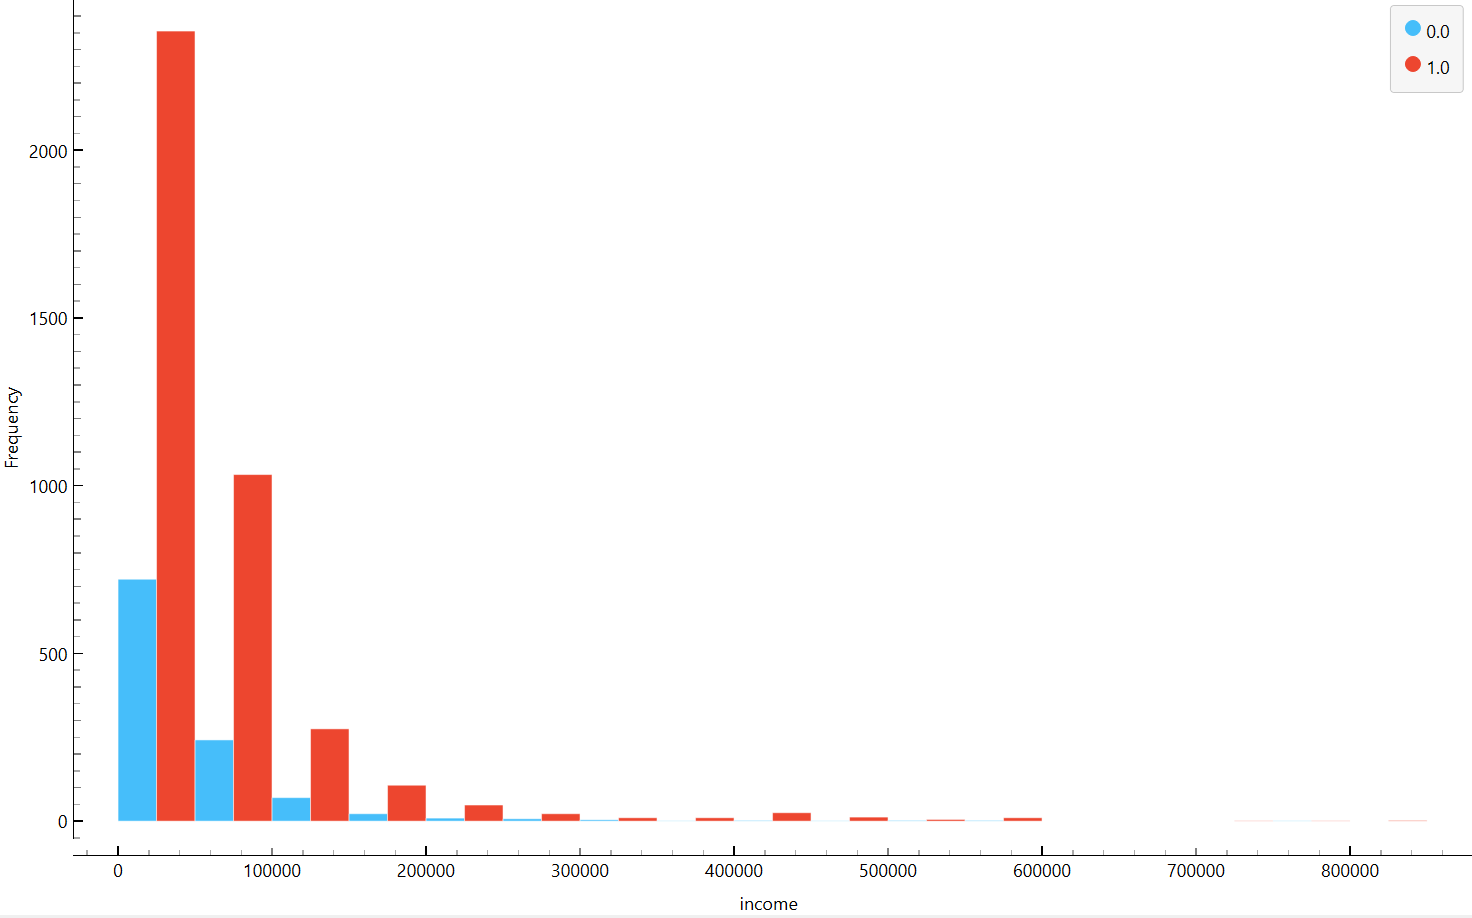
\includegraphics[width=\textwidth]{chapters/part 2 - images/income_race_distribution.png}
         \caption{Distribution of Race with Income.}
         \label{fig:income_race_dis}
     \end{subfigure}
     \hfill
     \begin{subfigure}[b]{0.45\textwidth}
         \centering
         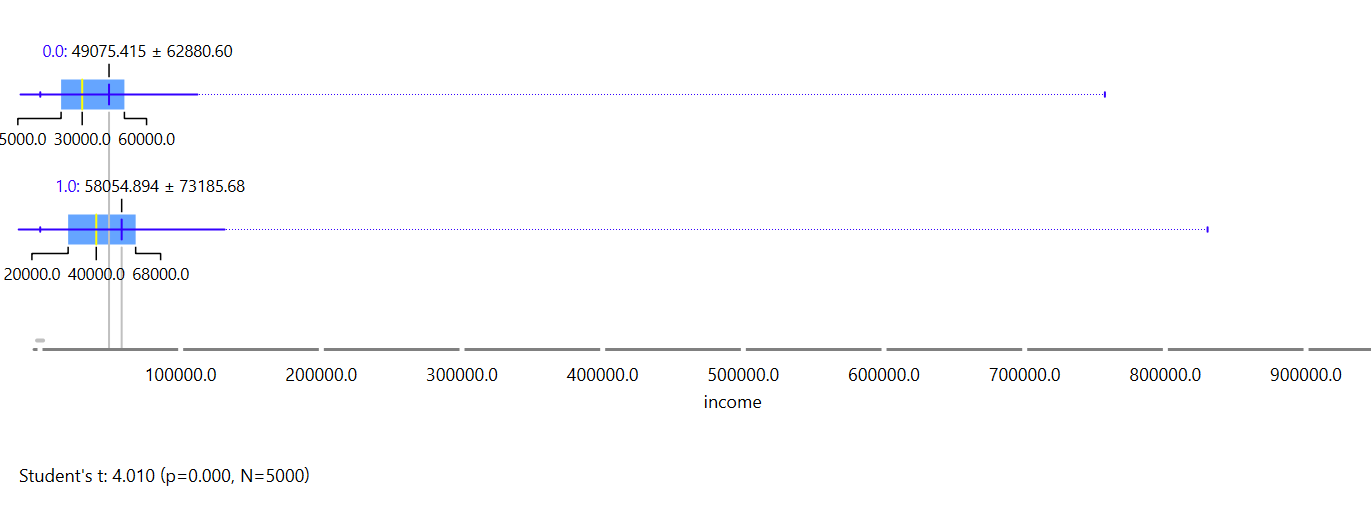
\includegraphics[width=\textwidth]{chapters/part 2 - images/income_race_box.png}
         \caption{Comparison of those how are White and those who are Not-white on average income}
         \label{fig:income_race_box}
     \end{subfigure}
     \caption{Effect of Race on Income (White=1, Other=0).}
     \label{fig:income_race_overview}
\end{figure}
Across all groups there are more White representatives. With a median difference of $\$10,000$ and $P < 0.05$, there is sufficient evidence
to suggest \textbf{race} is a significant predictor to income; but less than gender since the T-test ($4.04$) is lower. Furthermore, there
is also a greater inequality (range in income) within the \texttt{white} group, shown by the greater standard deviation $(\pm73K vs \pm62K)$.




\section{Does \textbf{Place of Birth} have an effect on Income?}
\begin{figure}[H]
     \centering
     \begin{subfigure}[b]{0.45\textwidth}
         \centering
         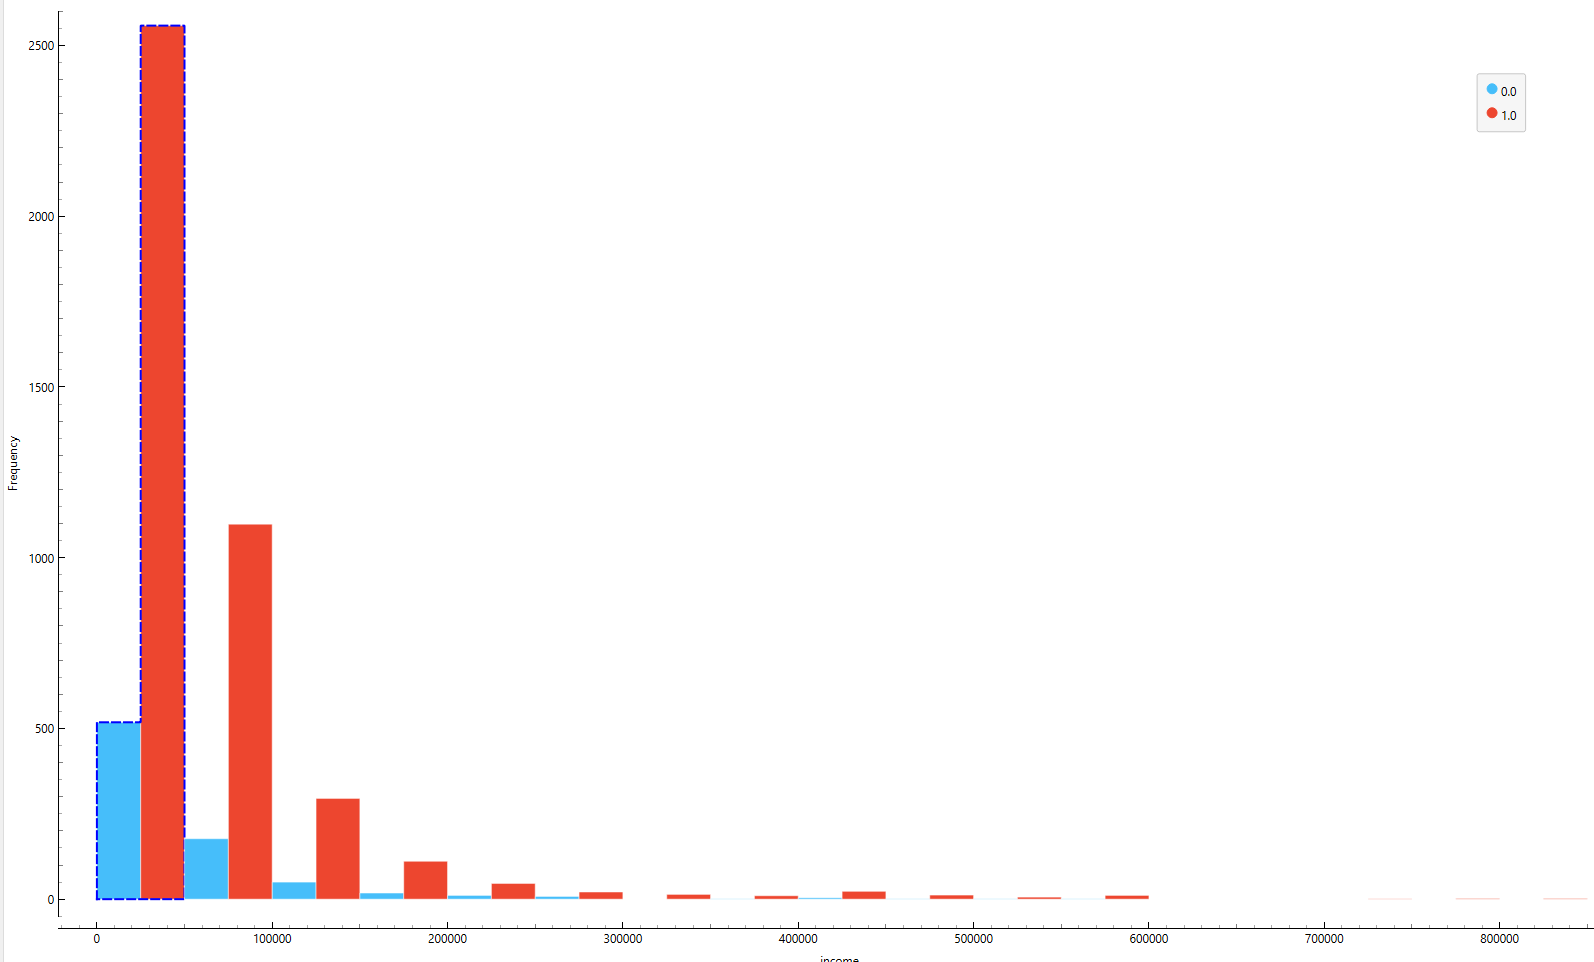
\includegraphics[width=\textwidth]{chapters/part 2 - images/income_US-POB_distribution.png}
         \caption{Distribution of Income with those born in the US.}
         \label{fig:income_POB_dis}
     \end{subfigure}
     \hfill
     \begin{subfigure}[b]{0.45\textwidth}
         \centering
         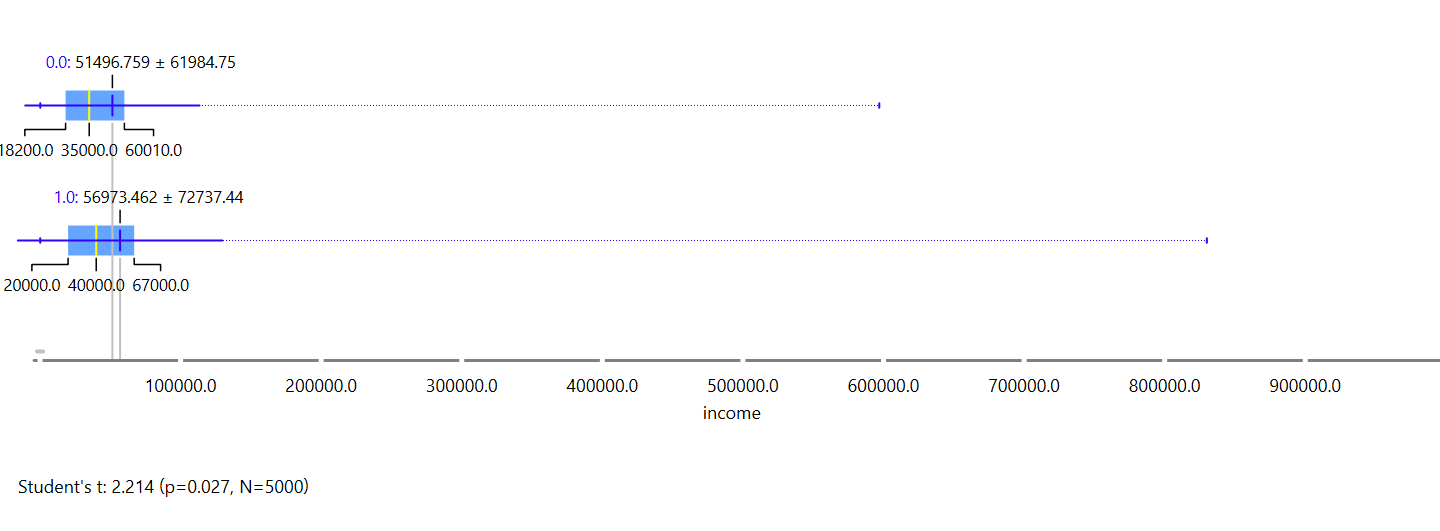
\includegraphics[width=\textwidth]{chapters/part 2 - images/income_US-POB_box.png}
         \caption{How does being born outside the US affect your income.}
         \label{fig:income_POB_box}
     \end{subfigure}
     \caption{Effect where you are born has on Income (US=1, Not-US=0).}
     \label{fig:income_POB_overview}
\end{figure}
Despite having the smallest $t$-statistic ($t=2.214$), a median difference of $\$5,000$ and $P < 0.05$ still provide sufficient evidence
to suggest that birth region significantly influences income. Furthermore, a $\$10,750$  difference in standard deviation suggests that
those born in the US experience higher income volatility and a wider range of financial outcomes compared to those born elsewhere.


\section{Personal and Professional Drivers of Income}

\subsection{Age}
\begin{figure}[H]
     \centering
     \begin{subfigure}[b]{0.48\textwidth}
         \centering
         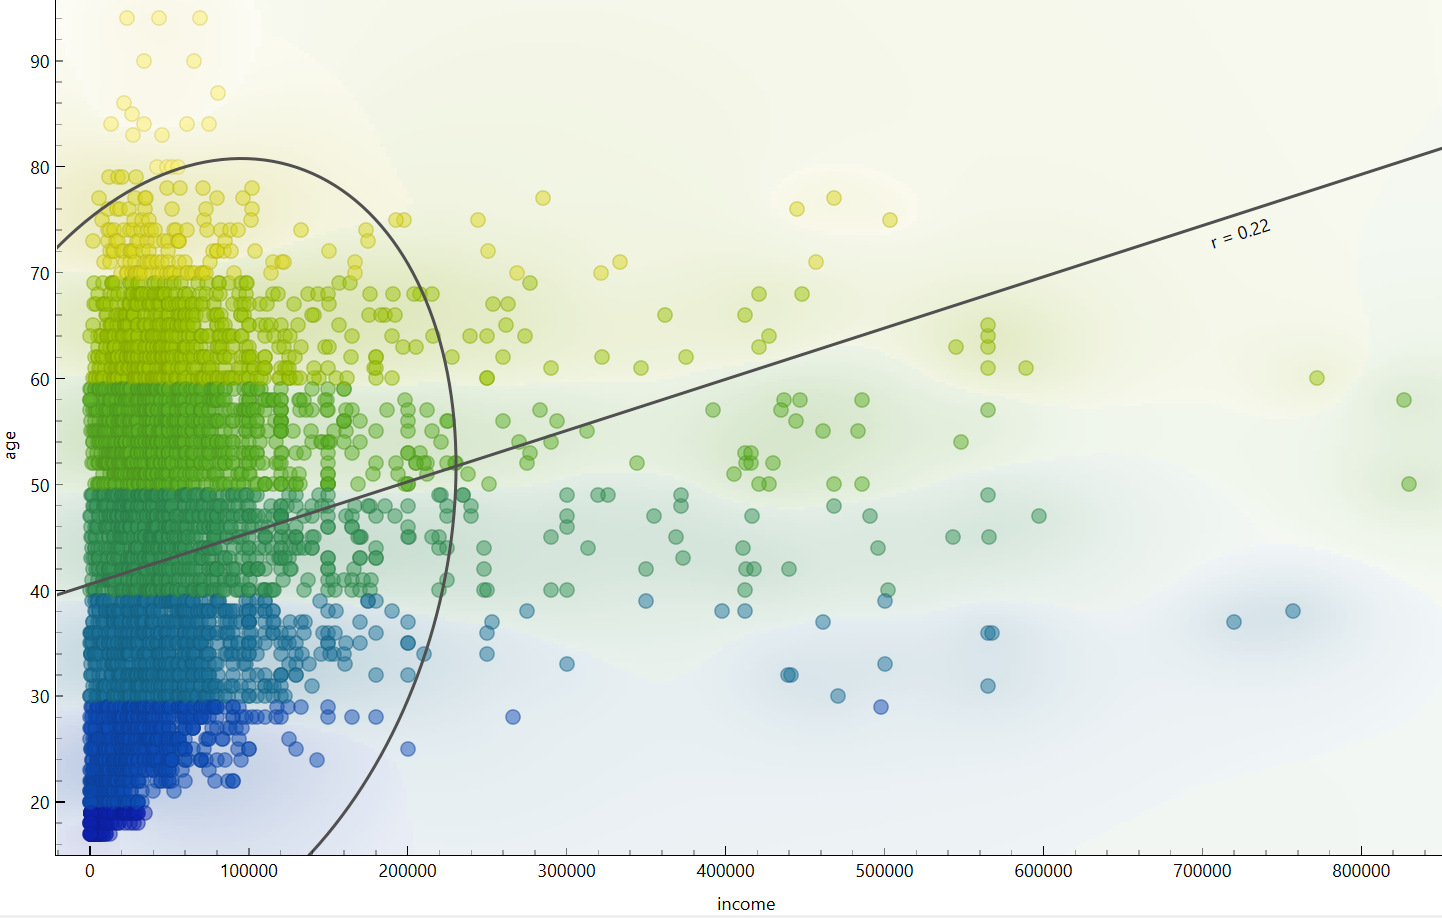
\includegraphics[width=\textwidth]{chapters/part 2 - images/income_age.png}
         \caption{Age vs. Raw Income}
         \label{fig:age_raw}
     \end{subfigure}
     \hfill
     \begin{subfigure}[b]{0.48\textwidth}
         \centering
         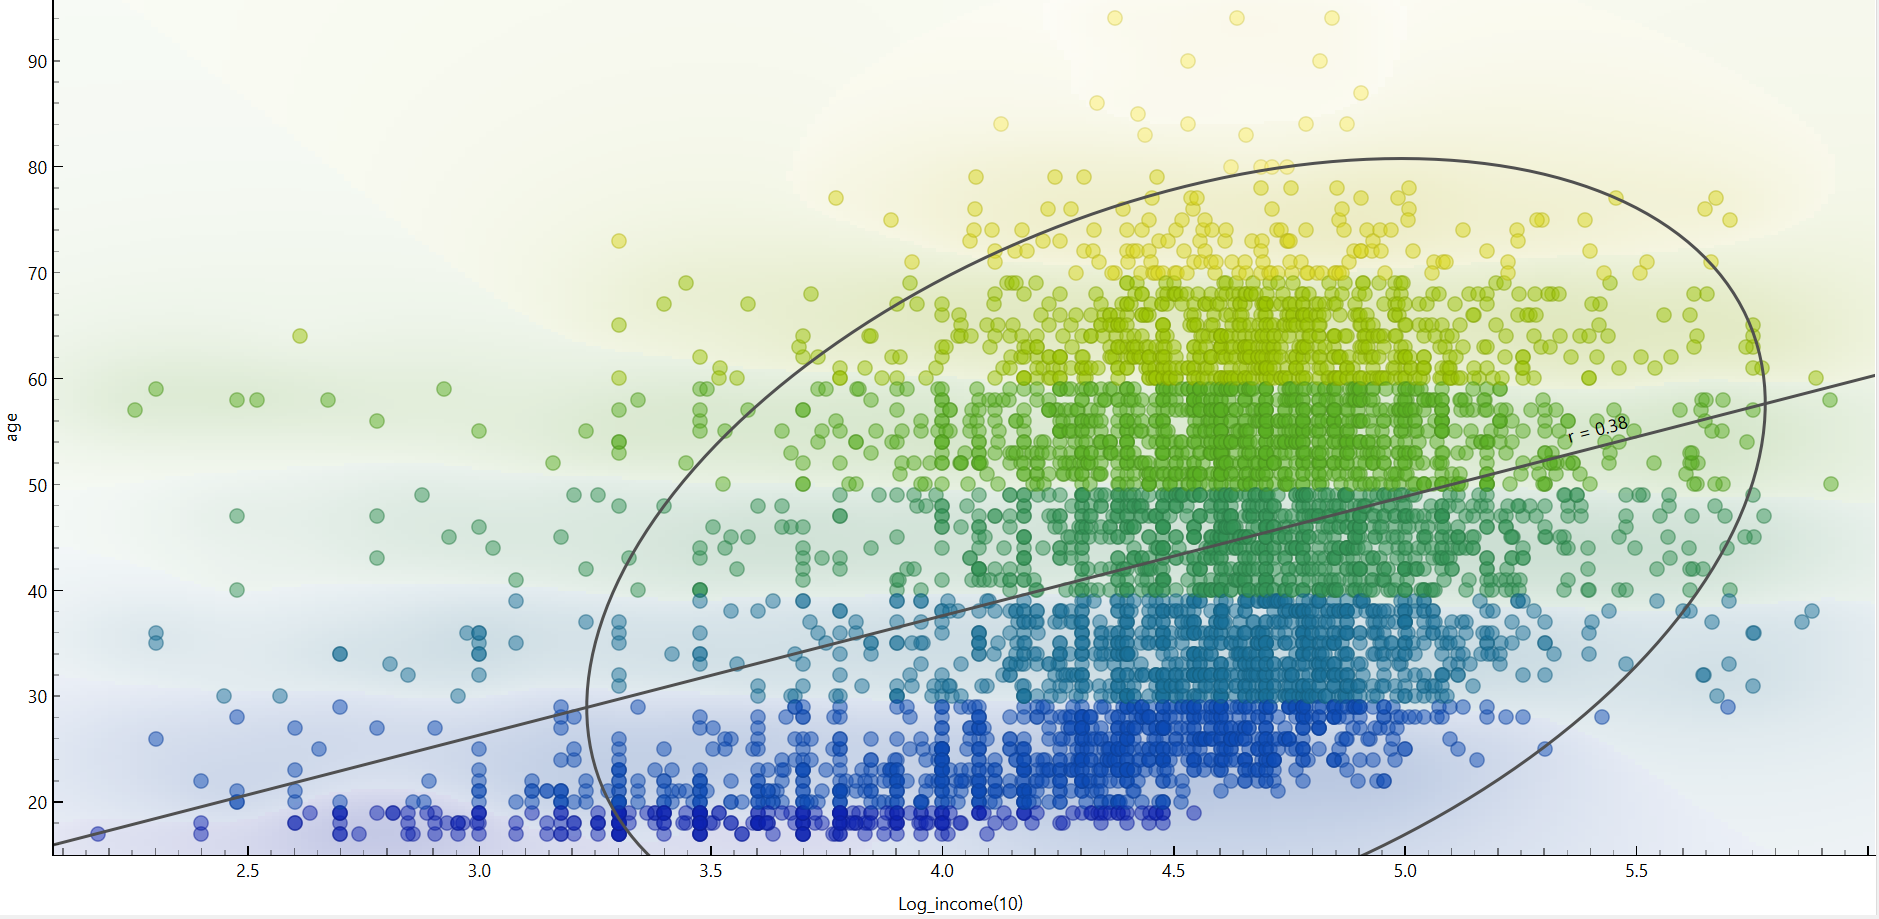
\includegraphics[width=\textwidth]{chapters/part 2 - images/income_age_log.png}
         \caption{Age vs. $\log_{10}(\text{income})$}
         \label{fig:age_log}
     \end{subfigure}
     \caption{Correlation between Age and Income metrics.}
\end{figure}
The raw data in Figure \ref{fig:age_raw} is difficult to interpret because the high-income outliers stretch the Y-axis, causing the
majority of data points to pool at the bottom. The log-transformed version (Figure \ref{fig:age_log}) is significantly better as it
linearises the growth trend. It suggests that as individuals age and gain experience, their earning potential increases, which is
reflected in a more consistent $R$ value and a clearer upward-sloping trend line.



\subsection{Education}
\label{sec:education_section}
\begin{figure}[H]
     \centering
     \begin{subfigure}[b]{0.48\textwidth}
         \centering
         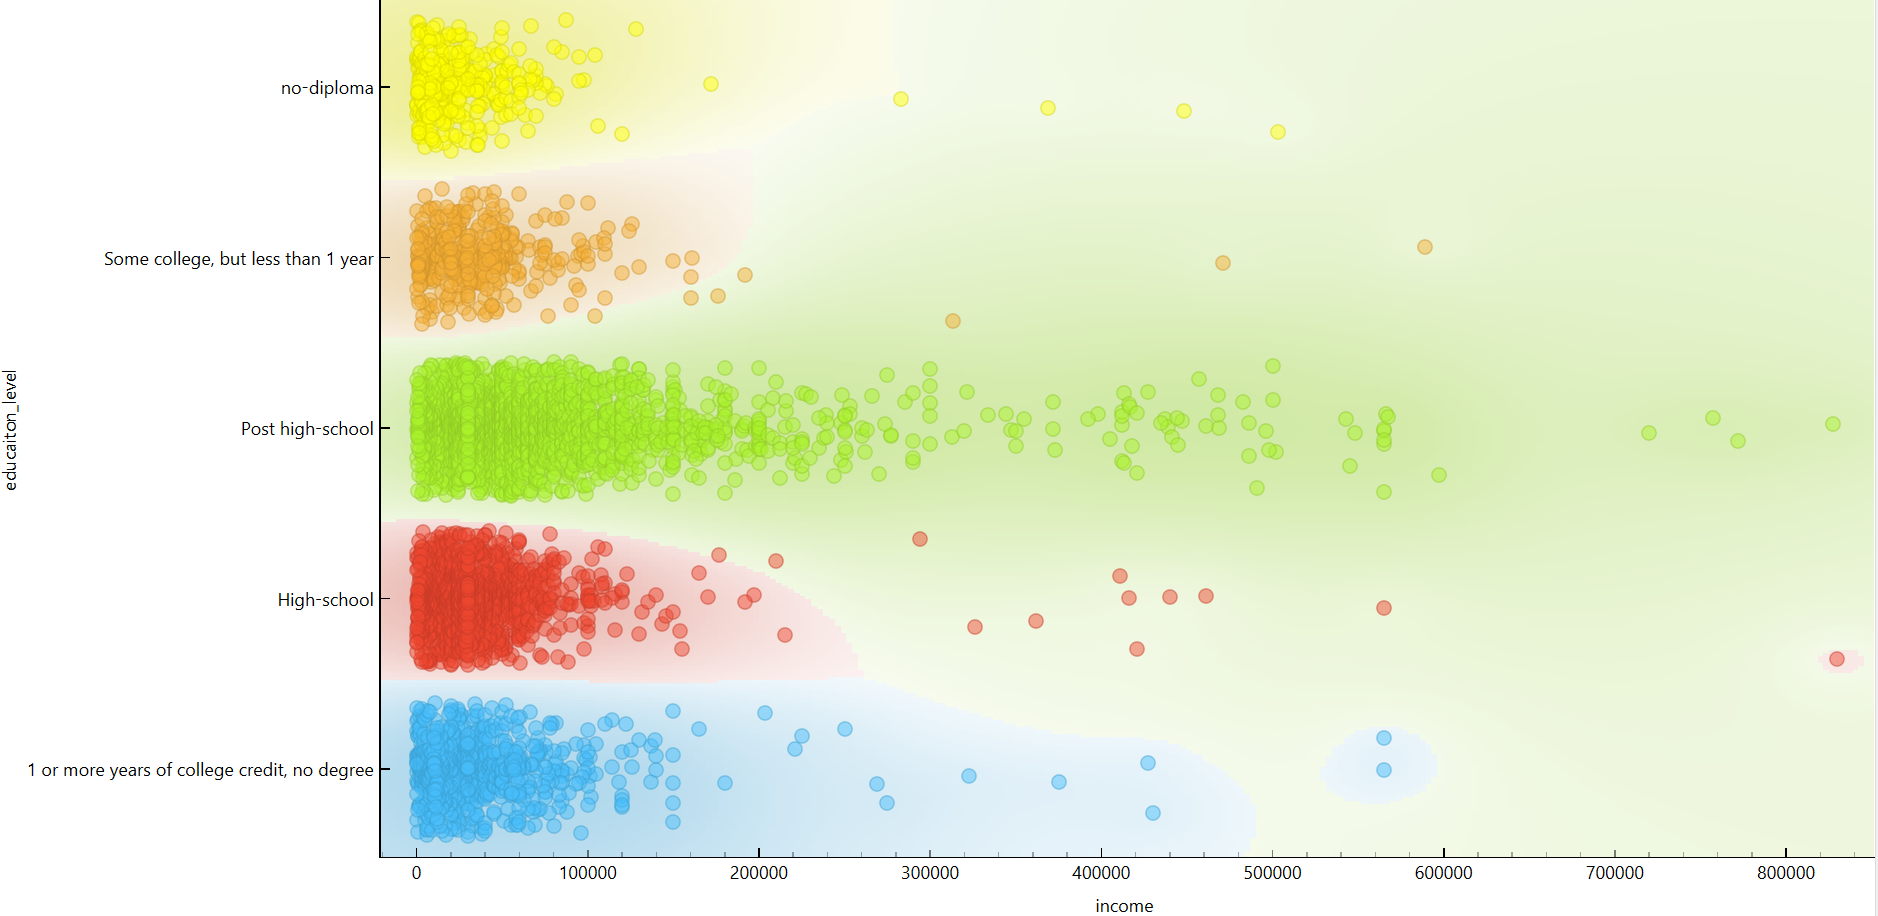
\includegraphics[width=\textwidth]{chapters/part 2 - images/income_education.png}
         \caption{Education vs. Raw Income}
         \label{fig:edu_raw}
     \end{subfigure}
     \hfill
     \begin{subfigure}[b]{0.48\textwidth}
         \centering
         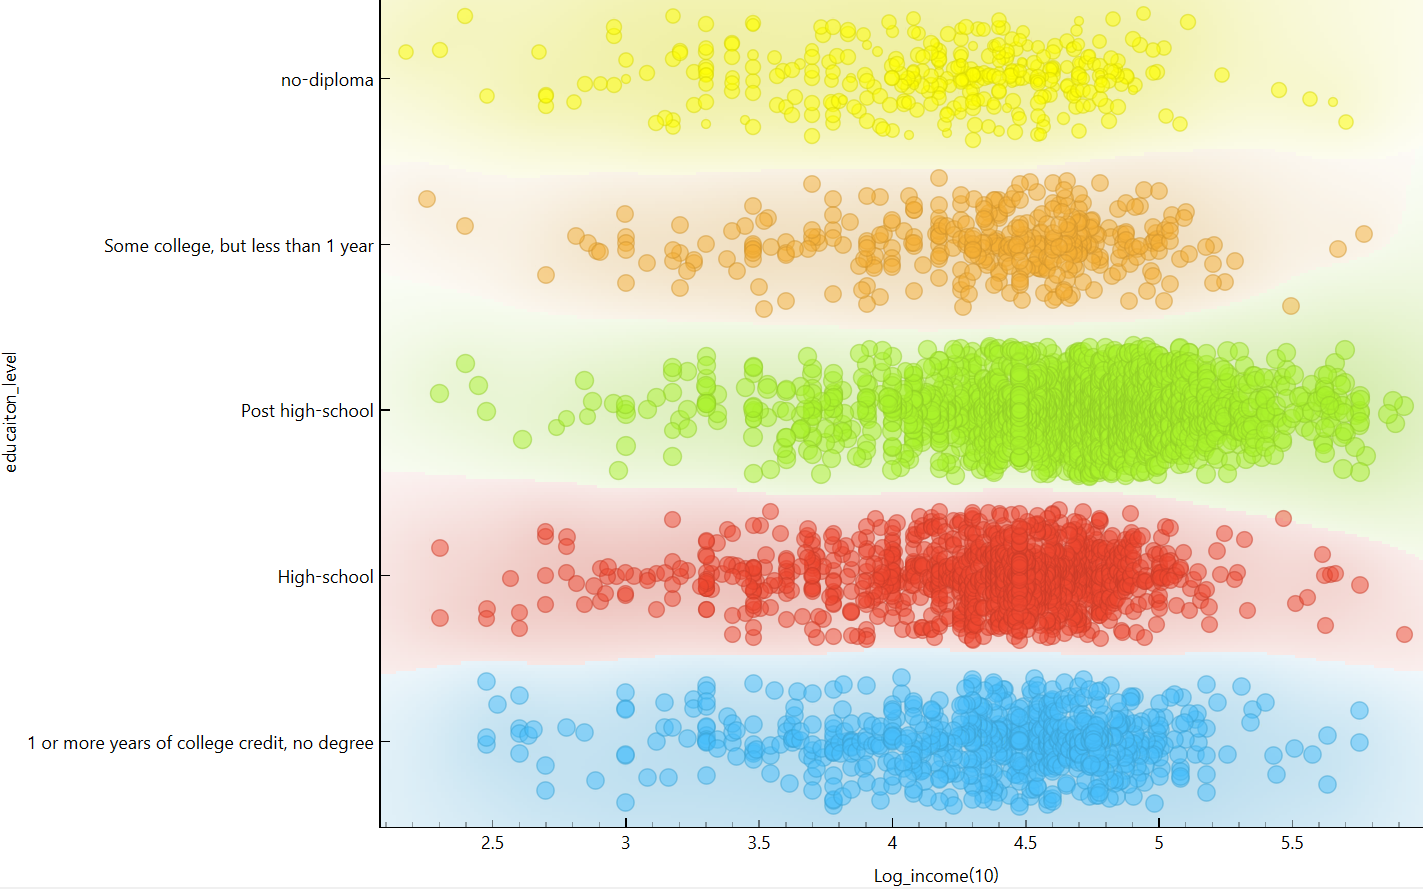
\includegraphics[width=\textwidth]{chapters/part 2 - images/income_education_log.png}
         \caption{Education vs. $\log_{10}(\text{income})$}
         \label{fig:edu_log}
     \end{subfigure}
     \caption{Correlation between Education level and Income metrics.}
\end{figure}
In the raw plot (Figure \ref{fig:edu_raw}), the extreme positive skew compresses the data, making central tendencies indistinguishable
beyond the lack of high-earners in the \texttt{no-diploma} group. Conversely, the $\log_{10}$ transformation (Figure \ref{fig:edu_log})
normalises this variance. Showing visibly that as duration in education increases, so does the general income cluster.



\subsection{Hours Worked}
\begin{figure}[H]
     \centering
     \begin{subfigure}[b]{0.48\textwidth}
         \centering
         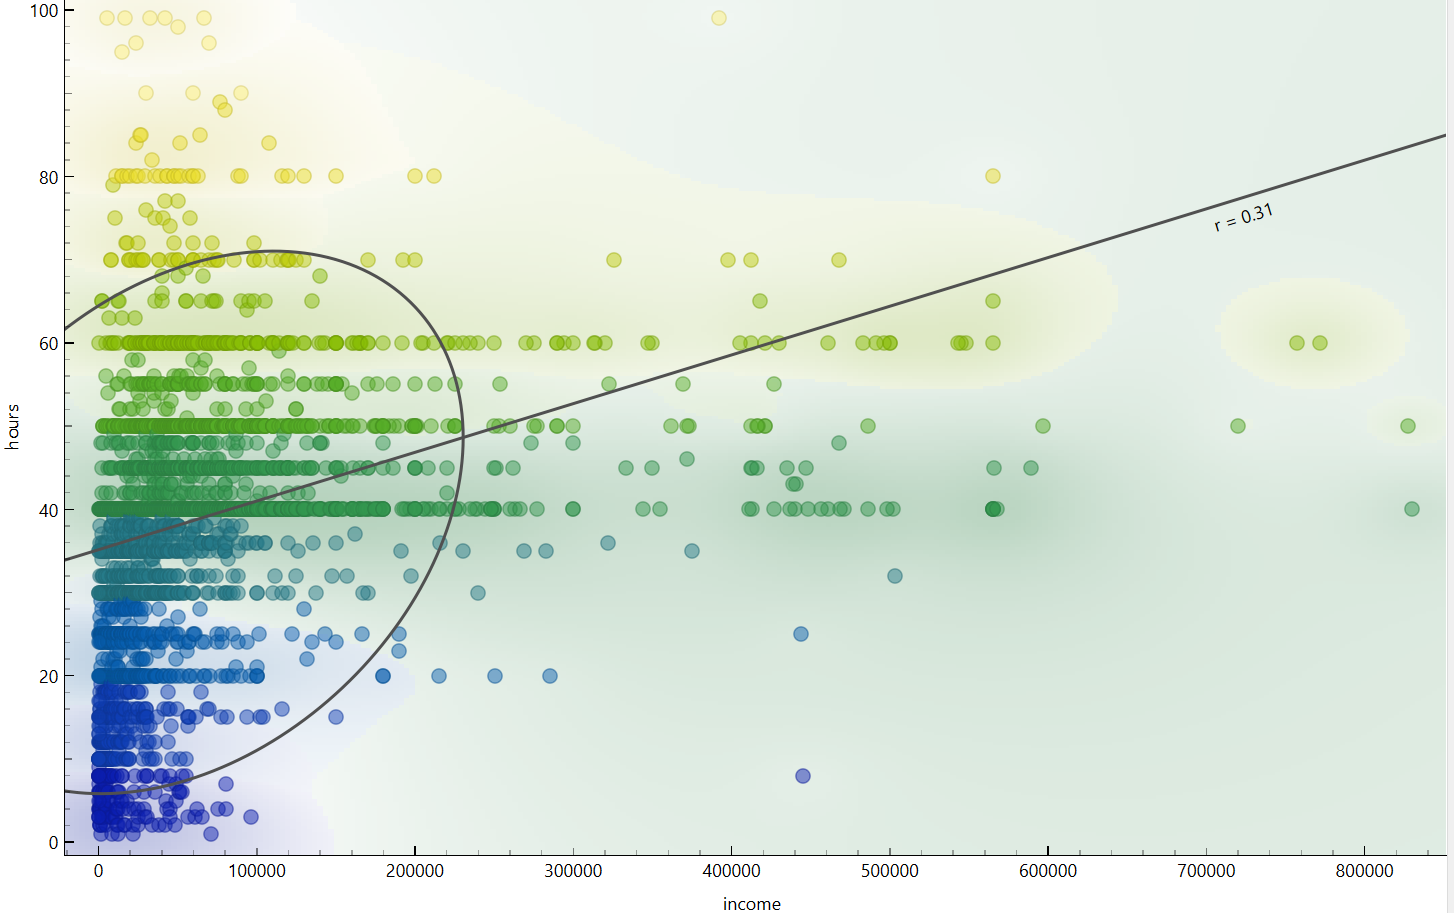
\includegraphics[width=\textwidth]{chapters/part 2 - images/income_hours.png}
         \caption{Hours vs. Raw Income}
         \label{fig:hours_raw}
     \end{subfigure}
     \hfill
     \begin{subfigure}[b]{0.48\textwidth}
         \centering
         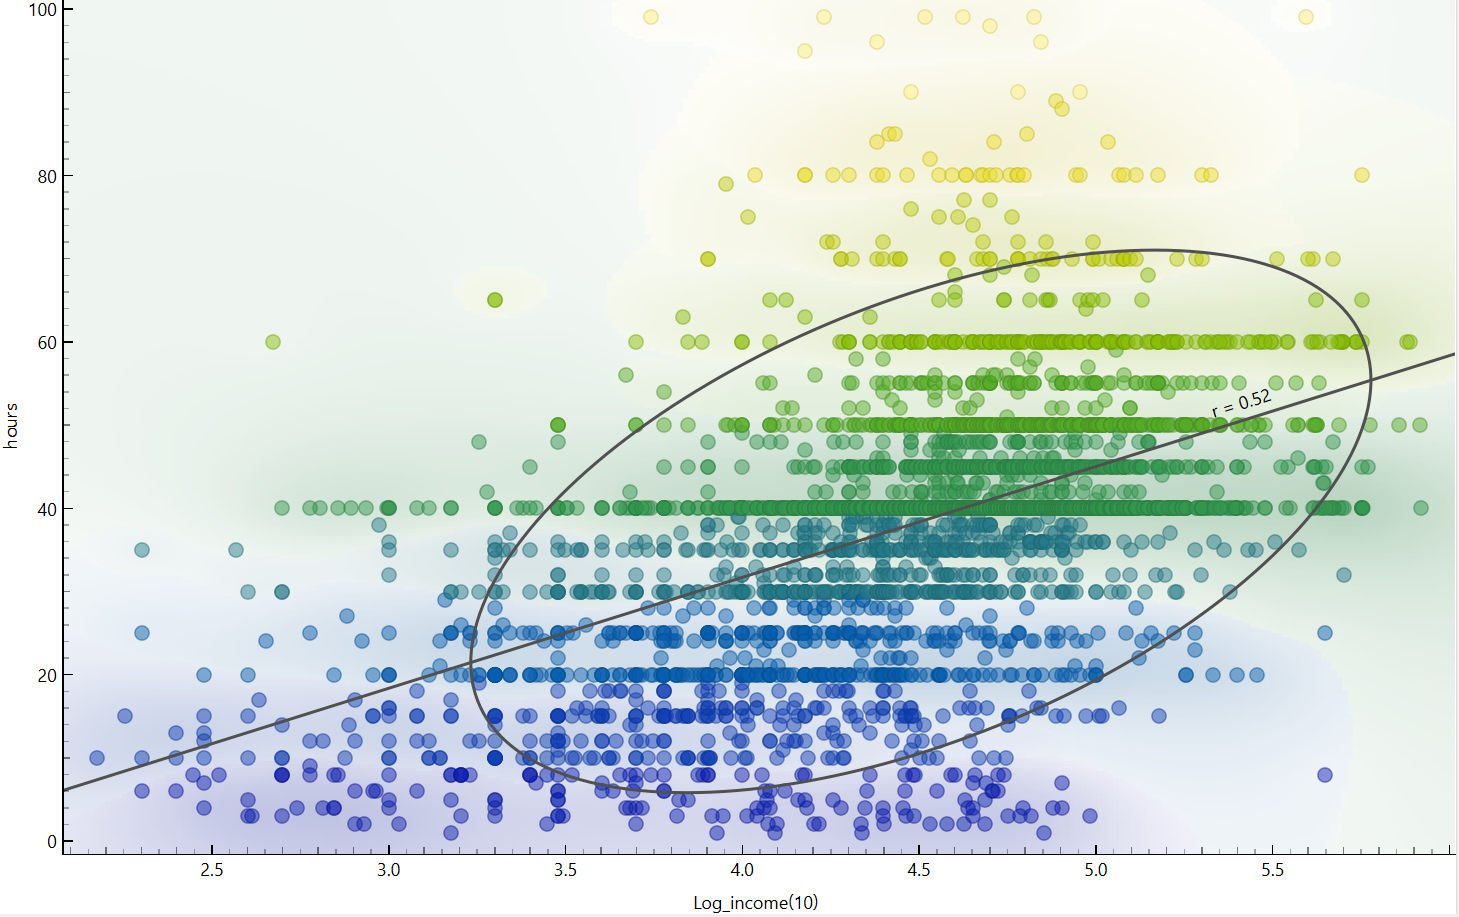
\includegraphics[width=\textwidth]{chapters/part 2 - images/income_hours_log.png}
         \caption{Hours vs. $\log_{10}(\text{income})$}
         \label{fig:hours_log}
     \end{subfigure}
     \caption{Correlation between Hours Worked and Income metrics.}
\end{figure}
While the relationship in Figure \ref{fig:hours_raw} is obscured by outliers the $\log_{10}$ transformation in Figure \ref{fig:hours_log}
reveals a clearer linear trend. A correlation of $R=0.52$ indicates a moderate positive linear relationship indicating hours worked
could be an appropriate predictor for income. The elliptical cluster also indicates that as hours increases, so does the income floor
(for most cases), with widening variance at higher earning levels.